\documentclass{../praktikum-protokollvorlage-latex/include/protokollclassE}
\SelectLanguage{english}

\newcommand{\praktikum}{P3}
\newcommand{\semester}{WS17/18}

\newcommand{\wochentag}{Mo}
\newcommand{\gruppennr}{106}

\newcommand{\nachnamea}{Elicabuk}
\newcommand{\vornamea}{Umut}
\newcommand{\nachnameb}{Pittermann}
\newcommand{\vornameb}{Martin}

\input{../common/emails.tex}

\hyphenation
{
	über-nom-me-nen
	an-ge-ge-be-nen
}

\newcommand{\maketitlepage}
{
	\begingroup \let\clearpage\relax
	\tableofcontents
	\listoffigures
	\listoftables
	\endgroup
}

\newcommand{\configureappendix}
{
	\chapter*{\appendixname} \addcontentsline{toc}{chapter}{\appendixname}
}

\newcommand{\s}[1]{\ensuremath{_\text{#1}}}


\newcommand{\versuch}{Angle Correlation}
\newcommand{\betreuer}{Arnaud Andrianavalomahefa}
\newcommand{\durchgefuehrt}{23.10.2017}

\newcommand{\abstract}{\ce{^{60}Co} decays by beta decay to the activated isotope \ce{^{60}Ni}. The activated nickel nucleus emits two gamma rays of energies \SI{1.17}{\MeV} and \SI{1.33}{\MeV}. Theory suggests that the successive gamma emissions must be distributed anisotropically. The angular correlation function and resolution time of coincidences are determined.} %The abstract
\begin{document}
	\FrontMatter
	\include{titlepage.ag}
	\maketitlepage

	\MainMatter

	\addchap{Prep}
\todo{no number or start at zero?}

This experiment validates \todo{actually validate and don't disprove} the anisotropy of the emission of gamma rays from excited nuclei states.
The angular distribution is dependent on the change of the magnetic quantum number between the inital and final states of the nucleus.
As the higher energy state has a spin number $j$ of at least one, there are multiple possible states which the excited nucleus can occupy.
At room temperature all possible states of the magnetic quantum number are populated equally, which results in an overall isotropic radiation pattern.

To isolate transitions with the same magnetic quantum number, a cascade of two transitions is observed, where the first transition leaves the nucleus in a defined state.
Naturally, the initial state also has multiple possible transitions which occur equally frequent, but the radiation pattern of the first transition is also anisotropic.

By selecting a nucleus with few enough states where there is a direction in which only one state emits radiation, it is possible use a first detector to detect this first gamma ray, confirming that the decaying nucleus is in the desired state, and observing the angular distribution with a second detector.

In this interpretation, the first detector also selects the quantization axis for the decay.
In reality, both detectors are interchangable.
Only the angle between the detectors is relevant for the analysis.

	\chapter{Introduction}
\begin{figure}
	\centering
	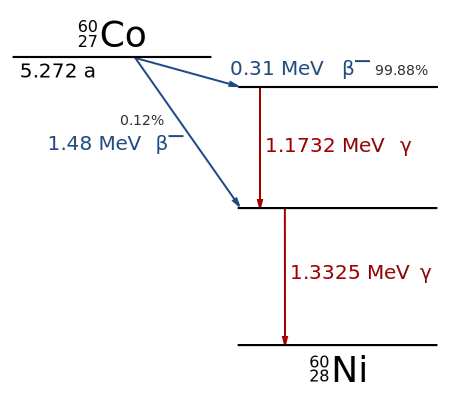
\includegraphics[width=.7\textwidth]{./img/co60_decay.pdf}
	\caption*{Source}
	\caption[The decay cascade of \ce{^{60}Co}]{\textbf{The decay cascade of \ce{^{60}Co}} After decaying from a 5+ spin state to a 4+ spin state of \ce{^{60}Ni} by beta decay with a probability of \num{99.88}\%, two gamma rays of energies \SI{1.17}{\MeV} and \SI{1.33}{\MeV} are emitted, each inhibting a spin of 2+.}
	\label{fig:co60_cascade}
\end{figure}
When the nucleus emits two gamma rays in a cascade, as shown in \autoref{fig:co60_cascade}, the spatial angular distribution of the second particle with respect to the first particle's direction of travel is anisotropic.
In particular, by detecting two particles of a cascade simultaneously, the equal engagement of states is removed, resulting in an anisotropy of the second particle.
The relative probability of the gamma particle's emission at an angle $\theta$ relative to the first photon is denoted as $W(\theta)$.
Normalizing this differential cross-section at $\theta=\SI{90}{\degree}$ yields the correlation function

\begin{equation*}
	K(\theta) &= 1 + \sum_{k}^{k_\text{max}}a_{2k}\cdot\cos^{2k}{\theta}.
\end{equation*}

The series terminates at $k_\text{max}=\min(I, L_1, L_2)=2$, where $I, L_1, L_2$ denote the nuclear spin after the first gamma emission and the angular momenta of both gamma rays respectively.
This results in the correlation function

\begin{equation}\label{eq:corr_func}
	K(\theta) &= 1 + a_2\cos^{2}{\theta} + a_4\cos^{4}{\theta},
\end{equation}
while only pure multipole orders (quadrupoles) are assumed.

	\chapter{Procedure}

\section{Geometry of the Setup}
\begin{figure}[tbp]
	\centering
	
\includegraphics[width=0.5\textwidth]{./img/setup.pdf}
	\caption[Geometry of the Setup]{\textbf{Geometry of the Setup} Detector $D_2$ moves between angles 180, 135 and 90 degrees, while detector $D_1$ is at a fixed position and defines the quantization axis.}
	\label{fig:setup}
\end{figure}
Yada yada setup as seen in \autoref{fig:setup}.

	\chapter{Data}

\section{Background}
\begin{table}
	\centering
	\caption[Background radiation]{\textbf{Background radiation}}
	\label{tab:background}
	\begin{tabular}{c|SSSS}
		\toprule
		background	&	{ch. 1 ev.}	&	{ch. 2 ev.}	&	{correlations}	&	{random coin.}	\\
		\midrule
			&	1181	&	1220	&	2.72	&	1.82	\\
		\bottomrule
	\end{tabular}
\end{table}

Background radiation data can be seen in \autoref{tab:background}, including distance corrections.
As data suggests, background radiation will not have a significant effect on the data.
In subsequent sections, background data will have been subtracted from measured quantities already.
\todo{Edit this. Blue book says different.}

\section{Measurement of $a_2$}

	\chapter{Results}
The experiment does not confirm the theory.
In general, the literature values do not lie within their respective error boundaries.
Both methods approximately yield the same error limits and values.
The considered errors turn out to be large in relation to their values.
However, keeping in mind that the error limits in method two can be minimized with increasing measurement time and series, one can obtain better certainty on the quantities to be determined.

Nevertheless, resolution time could be determined to lie within the calculated error boundaries, as the resolution time was defined to be \SI{200}{\ns}.

The fact that all established quantities do not resemble their respective literature values suggests two possible explanations:
Either the experiment was performed incorrectly, or the used equipment is faulty.
Considering \autoref{fig:e_spectrum}, one might notice the indistinct peaks and blurred slopes in the energy spectrum, which encourages the assumption that the second explanation might be more likely to be true.\todo{Just looking for excuses... :D}

The experiment can be improved by increasing the measurement time and checking the equipment.

	\Appendix
\configureappendix
\section{Data}
\setcounter{table}{0}
\def \hfillx {\hspace*{-\textwidth} \hfill}

\begin{table}[h]
	\caption{Eigenfrequencies: Monoatomic Chain, Series 1\&2}
	\label{tab:eigenfreq_a1_12a}
	\begin{tabular}{S|SS}
		\toprule
		{mode $n$}	&	{frequency $\omega_{n,\text{1}}$}	&	{frequency $\omega_{n,\text{2}}$} \\
		\midrule
		1	&	1.738	&	1.738	\\
		2	&	3.460	&	3.460	\\
		3	&	5.131	&	5.131	\\
		4	&	6.745	&	6.745	\\
		5	&	8.254	&	8.254	\\
		6	&	9.650	&	9.650	\\
		7	&	10.938	&	10.938	\\
		8	&	12.052	&	12.052	\\
		9	&	12.993	&	12.993	\\
		10	&	13.745	&	13.745	\\
		11	&	14.307	&	14.307	\\
		12	&	14.627	&	14.627	\\
		\bottomrule
	\end{tabular}
	\hfillx
	\begin{tabular}{S|SS}
		\toprule
		{mode $n$}	&	{frequency $\omega_{n,\text{1}}$}	&	{frequency $\omega_{n,\text{2}}$} \\
		\midrule
		1	&	1.740	&	1.740	\\
		2	&	3.456	&	3.456	\\
		3	&	5.130	&	5.130	\\
		4	&	6.733	&	6.733	\\
		5	&	8.246	&	8.246	\\
		6	&	9.643	&	9.643	\\
		7	&	10.927	&	10.927	\\
		8	&	12.039	&	12.039	\\
		9	&	12.979	&	12.979	\\
		10	&	13.734	&	13.734	\\
		11	&	14.299	&	14.299	\\
		12	&	14.613	&	14.613	\\
		\bottomrule
	\end{tabular}
\end{table}
\begin{table}[h]
	\caption{Eigenfrequencies: Monoatomic Chain, Series 3\&4}
	\label{tab:eigenfreq_a1_34a}
	\begin{tabular}{S|SS}
		\toprule
		{mode $n$}	&	{frequency $\omega_{n,\text{1}}$}	&	{frequency $\omega_{n,\text{2}}$} \\
		\midrule
		1	&	1.738	&	1.738	\\
		2	&	3.462	&	3.462	\\
		3	&	5.131	&	5.131	\\
		4	&	6.736	&	6.736	\\
		5	&	8.250	&	8.250	\\
		6	&	9.649	&	9.649	\\
		7	&	10.931	&	10.931	\\
		8	&	12.043	&	12.043	\\
		9	&	12.982	&	12.982	\\
		10	&	13.736	&	13.736	\\
		11	&	14.304	&	14.304	\\
		12	&	14.620	&	14.619	\\
		\bottomrule
	\end{tabular}
	\hfillx
	\begin{tabular}{S|SS}
		\toprule
		{mode $n$}	&	{frequency $\omega_{n,\text{1}}$}	&	{frequency $\omega_{n,\text{2}}$} \\
		\midrule
		1	&	1.742	&	1.742	\\
		2	&	3.460	&	3.460	\\
		3	&	5.134	&	5.134	\\
		4	&	6.739	&	6.739	\\
		5	&	8.252	&	8.252	\\
		6	&	9.647	&	9.647	\\
		7	&	10.929	&	10.930	\\
		8	&	12.050	&	12.050	\\
		9	&	12.985	&	12.985	\\
		10	&	13.745	&	13.745	\\
		11	&	14.306	&	14.306	\\
		12	&	14.620	&	14.621	\\
		\bottomrule
	\end{tabular}
\end{table}
\begin{table}[h]
	\caption{Eigenfrequencies: Biatomic Chain, Series 1\&2}
	\label{tab:eigenfreq_a1_12b}
	\begin{tabular}{S|SS}
		\toprule
		{excitation $n$}	&	{freq. $\omega_{n,\text{1}}$}	&	{freq. $\omega_{n,\text{2}}$} \\
		\midrule
		1	&	1.509	&	1.509	\\
		2	&	2.996	&	2.996	\\
		3	&	4.428	&	4.428	\\
		4	&	5.773	&	5.773	\\
		5	&	6.970	&	6.971	\\
		6	&	7.839	&	7.839	\\
		7	&	10.422	&	10.421	\\
		8	&	11.028	&	10.821	\\
		9	&	11.722	&	11.028	\\
		10	&	12.336	&	11.722	\\
		11	&	12.786	&	12.336	\\
		12	&	13.057	&	12.787	\\
		\bottomrule
	\end{tabular}
	\hfillx
	\begin{tabular}{S|SS}
		\toprule
		{excitation $n$}	&	{freq. $\omega_{n,\text{1}}$}	&	{freq. $\omega_{n,\text{2}}$} \\
		\midrule
		1	&	1.512	&	1.512	\\
		2	&	2.992	&	2.992	\\
		3	&	4.429	&	4.429	\\
		4	&	5.778	&	5.778	\\
		5	&	6.970	&	6.970	\\
		6	&	7.839	&	7.838	\\
		7	&	10.423	&	10.423	\\
		8	&	11.023	&	11.023	\\
		9	&	11.720	&	11.720	\\
		10	&	12.337	&	12.337	\\
		11	&	12.783	&	12.783	\\
		12	&	13.057	&	13.056	\\
		\bottomrule
	\end{tabular}
\end{table}
\begin{table}[h]
	\caption{Eigenfrequencies: Biatomic Chain, Series 3\&4}
	\label{tab:eigenfreq_a1_34b}
	\begin{tabular}{S|SS}
		\toprule
		{excitation $n$}	&	{freq. $\omega_{n,\text{1}}$}	&	{freq. $\omega_{n,\text{2}}$} \\
		\midrule
		1	&	1.509	&	1.509	\\
		2	&	2.997	&	2.997	\\
		3	&	4.427	&	4.427	\\
		4	&	5.778	&	5.778	\\
		5	&	6.974	&	6.974	\\
		6	&	7.840	&	7.840	\\
		7	&	10.426	&	10.426	\\
		8	&	11.030	&	11.030	\\
		9	&	11.723	&	11.723	\\
		10	&	12.334	&	12.334	\\
		11	&	12.783	&	12.783	\\
		12	&	13.057	&	13.057	\\
		\bottomrule
	\end{tabular}
	\hfillx
	\begin{tabular}{S|SS}
		\toprule
		{excitation $n$}	&	{freq. $\omega_{n,\text{1}}$}	&	{freq. $\omega_{n,\text{2}}$} \\
		\midrule
		1	&	1.513	&	1.513	\\
		2	&	2.998	&	2.998	\\
		3	&	4.429	&	4.429	\\
		4	&	5.775	&	5.775	\\
		5	&	6.975	&	6.975	\\
		6	&	7.840	&	7.840	\\
		7	&	10.427	&	10.427	\\
		8	&	11.027	&	11.027	\\
		9	&	11.728	&	11.728	\\
		10	&	12.337	&	12.337	\\
		11	&	12.790	&	12.790	\\
		12	&	13.060	&	13.060	\\
		\bottomrule
	\end{tabular}
\end{table}


\begin{table}[h]
	\caption{Amplitudes of Biatomic Chain, 5th and 6th thingmajig, Modes 1 to 4}

	\begin{tabular}{SS}
		\toprule
		{$A_{5,1}$}&
		{$A_{6,1}$}\\
		\midrule
		142.99&150.64\\
		142.99&150.64\\
		142.99&150.64\\
		142.99&150.64\\
		142.99&150.50\\
		142.99&150.64\\
		142.99&150.64\\
		142.99&150.64\\
		142.99&150.64\\
		142.99&150.64\\
		143.25&150.77\\
		143.25&150.50\\
		143.25&150.77\\
		142.99&150.64\\
		142.99&150.64\\
		143.25&150.64\\
		143.25&150.77\\
		143.25&150.91\\
		143.25&150.91\\
		\bottomrule
	\end{tabular}
	\hfillx
	\begin{tabular}{SS}
		\toprule
		{$A_{5,2}$}&
		{$A_{6,2}$}\\
		\midrule
		90.76&32.49\\
		90.76&32.49\\
		90.76&32.49\\
		90.76&32.49\\
		90.63&32.49\\
		90.49&32.36\\
		90.49&32.36\\
		90.49&32.36\\
		90.63&32.36\\
		90.63&32.22\\
		90.63&32.36\\
		90.63&32.22\\
		90.63&32.36\\
		90.63&32.36\\
		90.63&32.22\\
		90.63&32.36\\
		90.63&32.36\\
		90.63&32.36\\
		90.49&32.22\\
		\bottomrule
	\end{tabular}
	\hfillx
	\begin{tabular}{SS}
		\toprule
		{$A_{5,3}$}&
		{$A_{6,3}$}\\
		\midrule
		97.34&181.25\\
		97.61&181.25\\
		97.34&181.25\\
		97.07&180.98\\
		97.07&180.98\\
		96.80&180.44\\
		96.80&180.18\\
		96.67&180.18\\
		96.67&180.18\\
		96.53&180.04\\
		96.80&179.91\\
		97.07&179.77\\
		97.07&179.91\\
		97.07&179.91\\
		96.80&179.91\\
		96.80&180.04\\
		96.80&180.04\\
		96.80&180.04\\
		96.53&179.91\\
		\bottomrule
	\end{tabular}
	\hfillx
	\begin{tabular}{SS}
		\toprule
		{$A_{5,4}$}&
		{$A_{6,4}$}\\
		\midrule
		166.48&66.46\\
		169.84&71.69\\
		169.17&70.75\\
		166.48&67.00\\
		164.20&62.16\\
		164.87&63.24\\
		165.54&64.44\\
		167.02&68.61\\
		168.50&70.62\\
		168.50&69.95\\
		166.75&68.61\\
		165.68&65.25\\
		163.66&62.56\\
		166.21&65.12\\
		167.02&67.53\\
		167.82&69.01\\
		168.23&69.68\\
		168.09&69.01\\
		166.62&65.38\\
		\bottomrule
	\end{tabular}
\end{table}

\begin{table}[h]
	\caption{Amplitudes of Biatomic Chain, 5th and 6th thingmajig, Modes 5 to 8}

	\begin{tabular}{SS}
		\toprule
		{$A_{5,5}$}&
		{$A_{6,5}$}\\
		\midrule
		39.20&85.66\\
		39.07&86.19\\
		38.94&85.66\\
		38.94&85.93\\
		38.94&85.66\\
		39.07&85.79\\
		39.07&85.93\\
		39.34&85.79\\
		39.07&86.60\\
		39.20&86.33\\
		38.80&86.19\\
		39.20&85.93\\
		39.20&86.19\\
		39.07&86.33\\
		39.07&86.46\\
		39.34&86.06\\
		39.07&86.60\\
		39.47&86.33\\
		38.94&86.46\\
		\bottomrule
	\end{tabular}
	\hfillx
	\begin{tabular}{SS}
		\toprule
		{$A_{5,6}$}&
		{$A_{6,6}$}\\
		\midrule
		125.26&30.34\\
		124.59&30.34\\
		125.00&30.34\\
		124.06&30.34\\
		124.19&29.40\\
		124.73&29.54\\
		125.13&30.07\\
		125.67&30.48\\
		126.20&30.48\\
		125.80&29.81\\
		125.26&29.00\\
		125.67&29.67\\
		125.80&30.21\\
		126.61&29.81\\
		127.41&29.94\\
		127.81&30.48\\
		128.49&30.75\\
		128.89&31.42\\
		128.89&31.15\\
		\bottomrule
	\end{tabular}
	\hfillx
	\begin{tabular}{SS}
		\toprule
		{$A_{5,7}$}&
		{$A_{6,7}$}\\
		\midrule
		15.31&63.91\\
		15.31&63.50\\
		15.04&63.77\\
		15.57&64.04\\
		15.98&62.97\\
		14.23&63.50\\
		15.31&63.77\\
		15.31&62.83\\
		14.50&63.91\\
		15.98&63.37\\
		15.98&63.10\\
		14.23&63.64\\
		15.57&62.83\\
		15.57&62.70\\
		14.77&62.97\\
		14.77&62.43\\
		15.57&62.97\\
		15.44&63.77\\
		15.57&63.37\\
		\bottomrule
	\end{tabular}
	\hfillx
	\begin{tabular}{SS}
		\toprule
		{$A_{5,8}$}&
		{$A_{6,8}$}\\
		\midrule
		9.67&68.47\\
		8.86&67.53\\
		9.67&67.53\\
		8.46&67.53\\
		8.32&67.00\\
		9.26&65.92\\
		7.79&66.73\\
		7.79&66.06\\
		7.12&66.06\\
		5.91&66.46\\
		7.52&67.13\\
		9.26&68.34\\
		9.13&68.07\\
		9.13&67.67\\
		9.13&67.26\\
		9.13&67.13\\
		8.32&67.40\\
		8.86&67.13\\
		8.86&66.46\\
		\bottomrule
	\end{tabular}
\end{table}

\begin{table}[h]
	\caption{Amplitudes of Biatomic Chain, 5th and 6th thingmajig, Modes 9 to 12}

	\begin{tabular}{SS}
		\toprule
		{$A_{5,9}$}&
		{$A_{6,9}$}\\
		\midrule
		49.27&41.49\\
		49.27&41.49\\
		49.68&41.35\\
		49.54&41.08\\
		49.54&41.75\\
		49.81&41.89\\
		49.41&41.75\\
		49.68&41.89\\
		48.20&41.75\\
		49.41&40.95\\
		48.87&41.08\\
		48.74&40.95\\
		48.47&40.68\\
		48.74&39.88\\
		48.06&41.35\\
		49.41&42.02\\
		48.87&41.35\\
		49.14&40.95\\
		49.68&40.81\\
		\bottomrule
	\end{tabular}
	\hfillx
	\begin{tabular}{SS}
		\toprule
		{$A_{5,10}$}&
		{$A_{6,10}$}\\
		\midrule
		23.36&72.90\\
		22.82&72.63\\
		21.75&72.10\\
		21.75&71.69\\
		21.62&71.29\\
		22.29&71.69\\
		22.29&71.43\\
		21.48&71.56\\
		21.88&71.56\\
		21.48&71.56\\
		22.02&72.10\\
		21.75&71.83\\
		22.29&71.96\\
		22.56&71.83\\
		22.29&71.43\\
		22.29&71.83\\
		22.02&70.75\\
		22.02&71.43\\
		21.75&71.56\\
		\bottomrule
	\end{tabular}
	\hfillx
	\begin{tabular}{SS}
		\toprule
		{$A_{5,11}$}&
		{$A_{6,11}$}\\
		\midrule
		34.37&18.80\\
		34.37&19.06\\
		34.10&17.72\\
		34.91&18.66\\
		34.10&19.87\\
		33.83&18.53\\
		33.56&18.13\\
		33.70&18.53\\
		33.16&17.19\\
		33.43&18.26\\
		33.30&18.13\\
		33.56&17.59\\
		33.30&17.99\\
		33.83&17.72\\
		33.30&17.99\\
		33.30&18.26\\
		33.70&18.66\\
		33.56&18.26\\
		33.56&18.53\\
		\bottomrule
	\end{tabular}
	\hfillx
	\begin{tabular}{SS}
		\toprule
		{$A_{5,12}$}&
		{$A_{6,12}$}\\
		\midrule
		56.12&95.86\\
		56.25&95.46\\
		56.39&95.46\\
		55.85&95.19\\
		55.72&95.46\\
		56.39&95.86\\
		56.66&95.73\\
		56.39&95.73\\
		55.85&95.46\\
		55.85&94.92\\
		55.85&94.79\\
		55.58&94.92\\
		56.12&95.19\\
		55.85&94.92\\
		55.72&95.19\\
		56.12&95.06\\
		55.99&94.79\\
		55.45&94.52\\
		55.58&94.38\\
		\bottomrule
	\end{tabular}
\end{table}

	%\TheBibliography
\bibliographystyle{babalpha}
\bibliography{../common/lit}

\end{document}
